\documentclass{standalone}
\usepackage{tikz}
\usetikzlibrary{patterns}
\usetikzlibrary{arrows.meta}
\begin{document}
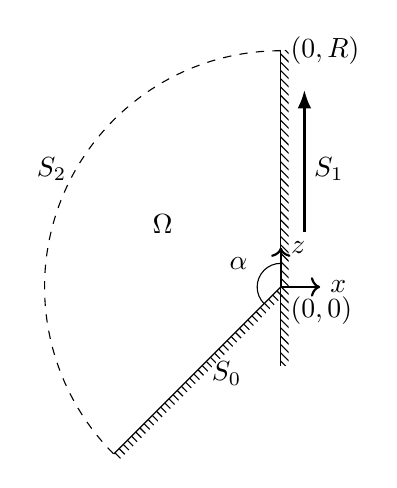
\begin{tikzpicture}
    
	\draw (1.5, 0.8) node{$\Omega$};
    
    \pattern [pattern=north west lines, rotate around={135:(3,0)}] (3,0) rectangle (2.9,3);
	\draw ({3.0*(1- sin(135))},{3.0*cos(135)}) -- (3.0,0.0);
	\draw (3.0-1, -1.1) node[below,right]{$S_0$};

	\draw (3.0,-1) -- (3.0, 3.0);
    \pattern[pattern=north west lines] (3,-1) rectangle (3.1,3);
	\draw[-{Latex},thick] (3.3,0.7) -- (3.3,2.5);
	\draw (3.3, 1.5) node[right]{$S_1$};
    
	\draw[dashed] (3.0, 3.0) arc (90:90+135:3.0);
	\draw (0.4, 1.5) node[left]{$S_2$};

	\draw (3.0 - 0.3, 0.3) node[left]{$\alpha$};
	\draw (3.0, 0.3) arc (90:90+135:0.3);
    
	%\draw[fill] (3.0, 0.0) circle (0.07);
	\draw[->,thick] (3,0) -- (3.5,0) node[right]{$x$};
	\draw[->,thick] (3,0) -- (3,0.5) node[right]{$z$};
	\draw (3.0, 0.0) node[below right]{$(0,0)$};
    
	\draw (3.0, 3.0) node[right]{$(0,R)$};


\end{tikzpicture}
\end{document}
